% Created by tikzDevice version 0.12.3.1 on 2022-07-25 14:53:08
% !TEX encoding = UTF-8 Unicode
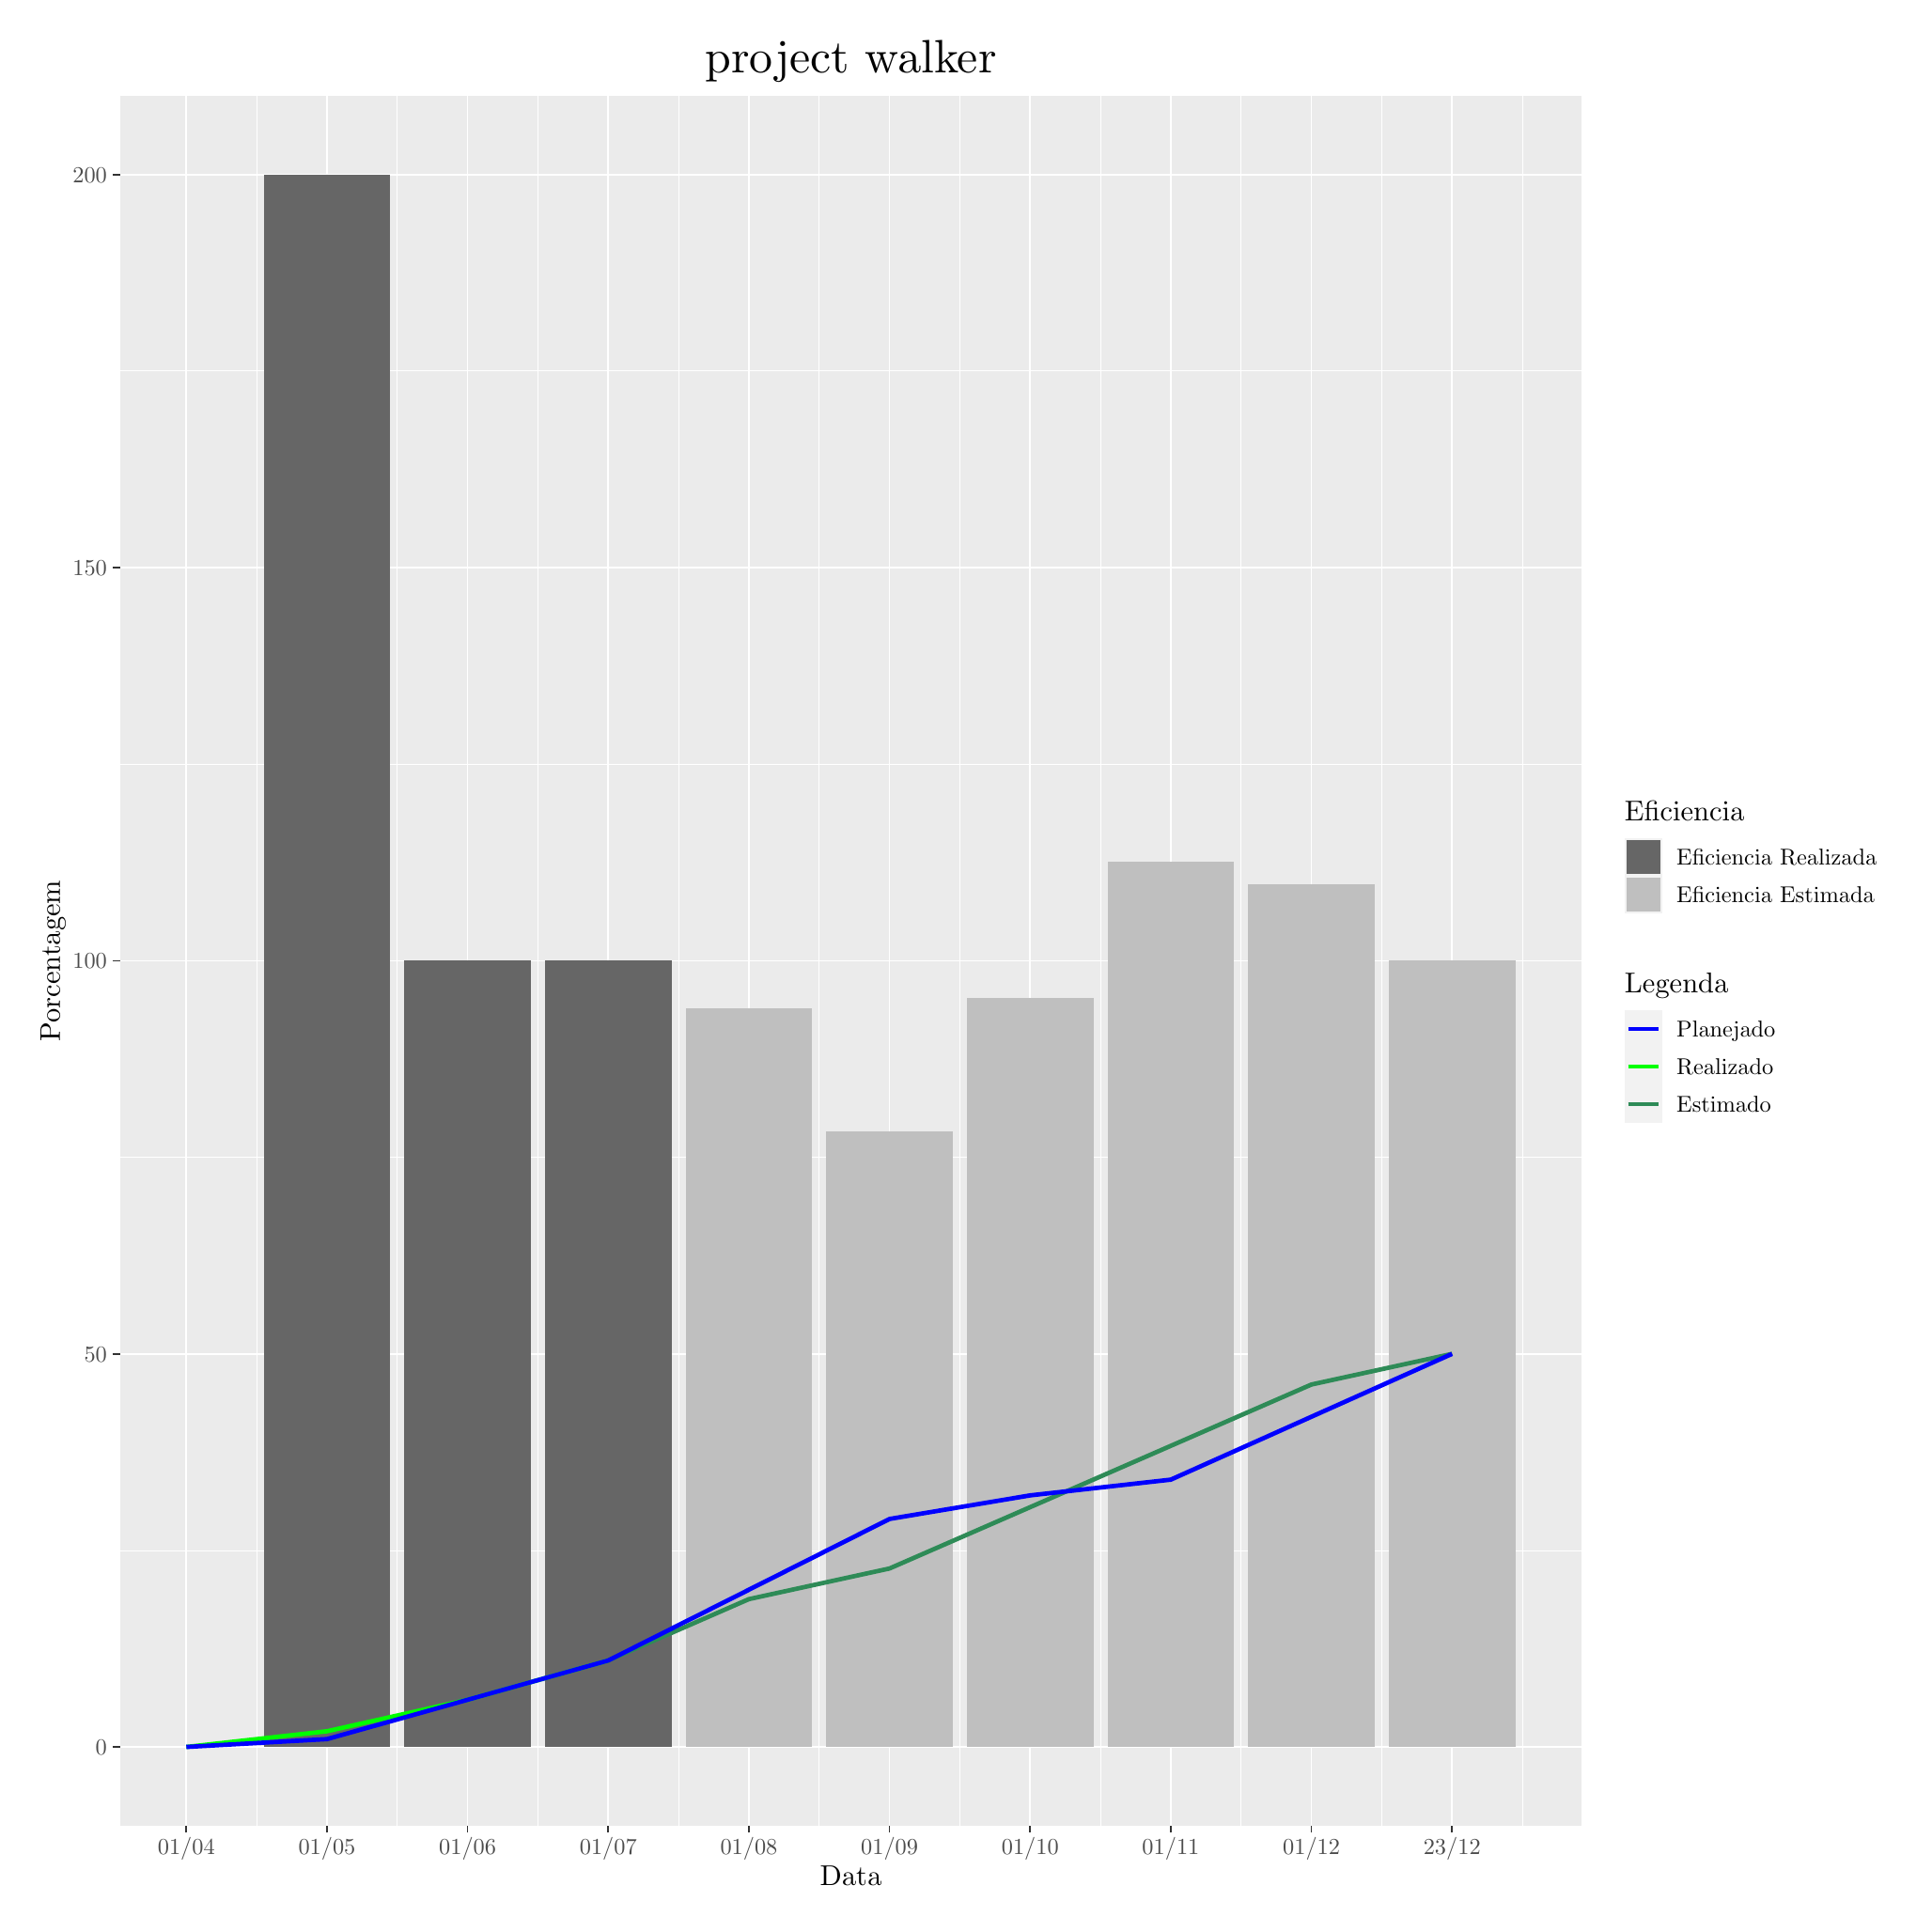
\begin{tikzpicture}[x=1pt,y=1pt]
\definecolor{fillColor}{RGB}{255,255,255}
\path[use as bounding box,fill=fillColor,fill opacity=0.00] (0,0) rectangle (722.70,722.70);
\begin{scope}
\path[clip] (  0.00,  0.00) rectangle (722.70,722.70);
\definecolor{drawColor}{RGB}{255,255,255}
\definecolor{fillColor}{RGB}{255,255,255}

\path[draw=drawColor,line width= 0.6pt,line join=round,line cap=round,fill=fillColor] (  0.00,  0.00) rectangle (722.70,722.70);
\end{scope}
\begin{scope}
\path[clip] ( 36.11, 30.69) rectangle (598.26,695.80);
\definecolor{fillColor}{gray}{0.92}

\path[fill=fillColor] ( 36.11, 30.69) rectangle (598.26,695.80);
\definecolor{drawColor}{RGB}{255,255,255}

\path[draw=drawColor,line width= 0.3pt,line join=round] ( 36.11,136.50) --
	(598.26,136.50);

\path[draw=drawColor,line width= 0.3pt,line join=round] ( 36.11,287.66) --
	(598.26,287.66);

\path[draw=drawColor,line width= 0.3pt,line join=round] ( 36.11,438.83) --
	(598.26,438.83);

\path[draw=drawColor,line width= 0.3pt,line join=round] ( 36.11,589.99) --
	(598.26,589.99);

\path[draw=drawColor,line width= 0.3pt,line join=round] ( 88.70, 30.69) --
	( 88.70,695.80);

\path[draw=drawColor,line width= 0.3pt,line join=round] (142.78, 30.69) --
	(142.78,695.80);

\path[draw=drawColor,line width= 0.3pt,line join=round] (196.86, 30.69) --
	(196.86,695.80);

\path[draw=drawColor,line width= 0.3pt,line join=round] (250.94, 30.69) --
	(250.94,695.80);

\path[draw=drawColor,line width= 0.3pt,line join=round] (305.02, 30.69) --
	(305.02,695.80);

\path[draw=drawColor,line width= 0.3pt,line join=round] (359.10, 30.69) --
	(359.10,695.80);

\path[draw=drawColor,line width= 0.3pt,line join=round] (413.18, 30.69) --
	(413.18,695.80);

\path[draw=drawColor,line width= 0.3pt,line join=round] (467.26, 30.69) --
	(467.26,695.80);

\path[draw=drawColor,line width= 0.3pt,line join=round] (521.34, 30.69) --
	(521.34,695.80);

\path[draw=drawColor,line width= 0.3pt,line join=round] (575.42, 30.69) --
	(575.42,695.80);

\path[draw=drawColor,line width= 0.6pt,line join=round] ( 36.11, 60.92) --
	(598.26, 60.92);

\path[draw=drawColor,line width= 0.6pt,line join=round] ( 36.11,212.08) --
	(598.26,212.08);

\path[draw=drawColor,line width= 0.6pt,line join=round] ( 36.11,363.24) --
	(598.26,363.24);

\path[draw=drawColor,line width= 0.6pt,line join=round] ( 36.11,514.41) --
	(598.26,514.41);

\path[draw=drawColor,line width= 0.6pt,line join=round] ( 36.11,665.57) --
	(598.26,665.57);

\path[draw=drawColor,line width= 0.6pt,line join=round] ( 61.66, 30.69) --
	( 61.66,695.80);

\path[draw=drawColor,line width= 0.6pt,line join=round] (115.74, 30.69) --
	(115.74,695.80);

\path[draw=drawColor,line width= 0.6pt,line join=round] (169.82, 30.69) --
	(169.82,695.80);

\path[draw=drawColor,line width= 0.6pt,line join=round] (223.90, 30.69) --
	(223.90,695.80);

\path[draw=drawColor,line width= 0.6pt,line join=round] (277.98, 30.69) --
	(277.98,695.80);

\path[draw=drawColor,line width= 0.6pt,line join=round] (332.06, 30.69) --
	(332.06,695.80);

\path[draw=drawColor,line width= 0.6pt,line join=round] (386.14, 30.69) --
	(386.14,695.80);

\path[draw=drawColor,line width= 0.6pt,line join=round] (440.22, 30.69) --
	(440.22,695.80);

\path[draw=drawColor,line width= 0.6pt,line join=round] (494.30, 30.69) --
	(494.30,695.80);

\path[draw=drawColor,line width= 0.6pt,line join=round] (548.38, 30.69) --
	(548.38,695.80);
\definecolor{fillColor}{gray}{0.40}

\path[fill=fillColor] ( 91.41, 60.92) rectangle (140.08,665.57);

\path[fill=fillColor] (145.49, 60.92) rectangle (194.16,363.24);

\path[fill=fillColor] (199.57, 60.92) rectangle (248.24,363.24);
\definecolor{fillColor}{gray}{0.75}

\path[fill=fillColor] (253.64, 60.92) rectangle (302.32,345.11);

\path[fill=fillColor] (307.72, 60.92) rectangle (356.40,297.57);

\path[fill=fillColor] (361.80, 60.92) rectangle (410.47,349.07);

\path[fill=fillColor] (415.88, 60.92) rectangle (464.55,401.48);

\path[fill=fillColor] (469.96, 60.92) rectangle (518.63,392.76);

\path[fill=fillColor] (524.04, 60.92) rectangle (572.71,363.24);
\definecolor{drawColor}{RGB}{46,139,87}

\path[draw=drawColor,line width= 1.7pt,line join=round] (223.90, 94.17) --
	(277.98,117.76) --
	(332.06,129.55) --
	(386.14,153.13) --
	(440.22,176.71) --
	(494.30,200.29) --
	(548.38,212.08);
\definecolor{drawColor}{RGB}{0,255,0}

\path[draw=drawColor,line width= 1.7pt,line join=round] ( 61.66, 60.92) --
	(115.74, 66.96) --
	(169.82, 79.06) --
	(223.90, 94.17);
\definecolor{drawColor}{RGB}{0,0,255}

\path[draw=drawColor,line width= 1.7pt,line join=round] ( 61.66, 60.92) --
	(115.74, 63.94) --
	(169.82, 79.06) --
	(223.90, 94.17) --
	(277.98,121.38) --
	(332.06,148.59) --
	(386.14,157.66) --
	(440.22,163.71) --
	(494.30,187.90) --
	(548.38,212.08);
\end{scope}
\begin{scope}
\path[clip] (  0.00,  0.00) rectangle (722.70,722.70);
\definecolor{drawColor}{gray}{0.30}

\node[text=drawColor,anchor=base east,inner sep=0pt, outer sep=0pt, scale=  0.88] at ( 31.16, 57.89) {0};

\node[text=drawColor,anchor=base east,inner sep=0pt, outer sep=0pt, scale=  0.88] at ( 31.16,209.05) {50};

\node[text=drawColor,anchor=base east,inner sep=0pt, outer sep=0pt, scale=  0.88] at ( 31.16,360.21) {100};

\node[text=drawColor,anchor=base east,inner sep=0pt, outer sep=0pt, scale=  0.88] at ( 31.16,511.38) {150};

\node[text=drawColor,anchor=base east,inner sep=0pt, outer sep=0pt, scale=  0.88] at ( 31.16,662.54) {200};
\end{scope}
\begin{scope}
\path[clip] (  0.00,  0.00) rectangle (722.70,722.70);
\definecolor{drawColor}{gray}{0.20}

\path[draw=drawColor,line width= 0.6pt,line join=round] ( 33.36, 60.92) --
	( 36.11, 60.92);

\path[draw=drawColor,line width= 0.6pt,line join=round] ( 33.36,212.08) --
	( 36.11,212.08);

\path[draw=drawColor,line width= 0.6pt,line join=round] ( 33.36,363.24) --
	( 36.11,363.24);

\path[draw=drawColor,line width= 0.6pt,line join=round] ( 33.36,514.41) --
	( 36.11,514.41);

\path[draw=drawColor,line width= 0.6pt,line join=round] ( 33.36,665.57) --
	( 36.11,665.57);
\end{scope}
\begin{scope}
\path[clip] (  0.00,  0.00) rectangle (722.70,722.70);
\definecolor{drawColor}{gray}{0.20}

\path[draw=drawColor,line width= 0.6pt,line join=round] ( 61.66, 27.94) --
	( 61.66, 30.69);

\path[draw=drawColor,line width= 0.6pt,line join=round] (115.74, 27.94) --
	(115.74, 30.69);

\path[draw=drawColor,line width= 0.6pt,line join=round] (169.82, 27.94) --
	(169.82, 30.69);

\path[draw=drawColor,line width= 0.6pt,line join=round] (223.90, 27.94) --
	(223.90, 30.69);

\path[draw=drawColor,line width= 0.6pt,line join=round] (277.98, 27.94) --
	(277.98, 30.69);

\path[draw=drawColor,line width= 0.6pt,line join=round] (332.06, 27.94) --
	(332.06, 30.69);

\path[draw=drawColor,line width= 0.6pt,line join=round] (386.14, 27.94) --
	(386.14, 30.69);

\path[draw=drawColor,line width= 0.6pt,line join=round] (440.22, 27.94) --
	(440.22, 30.69);

\path[draw=drawColor,line width= 0.6pt,line join=round] (494.30, 27.94) --
	(494.30, 30.69);

\path[draw=drawColor,line width= 0.6pt,line join=round] (548.38, 27.94) --
	(548.38, 30.69);
\end{scope}
\begin{scope}
\path[clip] (  0.00,  0.00) rectangle (722.70,722.70);
\definecolor{drawColor}{gray}{0.30}

\node[text=drawColor,anchor=base,inner sep=0pt, outer sep=0pt, scale=  0.88] at ( 61.66, 19.68) {01/04};

\node[text=drawColor,anchor=base,inner sep=0pt, outer sep=0pt, scale=  0.88] at (115.74, 19.68) {01/05};

\node[text=drawColor,anchor=base,inner sep=0pt, outer sep=0pt, scale=  0.88] at (169.82, 19.68) {01/06};

\node[text=drawColor,anchor=base,inner sep=0pt, outer sep=0pt, scale=  0.88] at (223.90, 19.68) {01/07};

\node[text=drawColor,anchor=base,inner sep=0pt, outer sep=0pt, scale=  0.88] at (277.98, 19.68) {01/08};

\node[text=drawColor,anchor=base,inner sep=0pt, outer sep=0pt, scale=  0.88] at (332.06, 19.68) {01/09};

\node[text=drawColor,anchor=base,inner sep=0pt, outer sep=0pt, scale=  0.88] at (386.14, 19.68) {01/10};

\node[text=drawColor,anchor=base,inner sep=0pt, outer sep=0pt, scale=  0.88] at (440.22, 19.68) {01/11};

\node[text=drawColor,anchor=base,inner sep=0pt, outer sep=0pt, scale=  0.88] at (494.30, 19.68) {01/12};

\node[text=drawColor,anchor=base,inner sep=0pt, outer sep=0pt, scale=  0.88] at (548.38, 19.68) {23/12};
\end{scope}
\begin{scope}
\path[clip] (  0.00,  0.00) rectangle (722.70,722.70);
\definecolor{drawColor}{RGB}{0,0,0}

\node[text=drawColor,anchor=base,inner sep=0pt, outer sep=0pt, scale=  1.10] at (317.19,  7.64) {Data};
\end{scope}
\begin{scope}
\path[clip] (  0.00,  0.00) rectangle (722.70,722.70);
\definecolor{drawColor}{RGB}{0,0,0}

\node[text=drawColor,rotate= 90.00,anchor=base,inner sep=0pt, outer sep=0pt, scale=  1.10] at ( 13.08,363.24) {Porcentagem};
\end{scope}
\begin{scope}
\path[clip] (  0.00,  0.00) rectangle (722.70,722.70);
\definecolor{fillColor}{RGB}{255,255,255}

\path[fill=fillColor] (609.26,375.97) rectangle (717.20,431.09);
\end{scope}
\begin{scope}
\path[clip] (  0.00,  0.00) rectangle (722.70,722.70);
\definecolor{drawColor}{RGB}{0,0,0}

\node[text=drawColor,anchor=base west,inner sep=0pt, outer sep=0pt, scale=  1.10] at (614.76,416.95) {Eficiencia};
\end{scope}
\begin{scope}
\path[clip] (  0.00,  0.00) rectangle (722.70,722.70);
\definecolor{fillColor}{gray}{0.95}

\path[fill=fillColor] (614.76,395.93) rectangle (629.22,410.38);
\end{scope}
\begin{scope}
\path[clip] (  0.00,  0.00) rectangle (722.70,722.70);
\definecolor{fillColor}{gray}{0.40}

\path[fill=fillColor] (615.48,396.64) rectangle (628.51,409.67);
\end{scope}
\begin{scope}
\path[clip] (  0.00,  0.00) rectangle (722.70,722.70);
\definecolor{fillColor}{gray}{0.40}

\path[fill=fillColor] (615.48,396.64) rectangle (628.51,409.67);
\end{scope}
\begin{scope}
\path[clip] (  0.00,  0.00) rectangle (722.70,722.70);
\definecolor{fillColor}{gray}{0.95}

\path[fill=fillColor] (614.76,381.47) rectangle (629.22,395.93);
\end{scope}
\begin{scope}
\path[clip] (  0.00,  0.00) rectangle (722.70,722.70);
\definecolor{fillColor}{gray}{0.75}

\path[fill=fillColor] (615.48,382.18) rectangle (628.51,395.21);
\end{scope}
\begin{scope}
\path[clip] (  0.00,  0.00) rectangle (722.70,722.70);
\definecolor{fillColor}{gray}{0.75}

\path[fill=fillColor] (615.48,382.18) rectangle (628.51,395.21);
\end{scope}
\begin{scope}
\path[clip] (  0.00,  0.00) rectangle (722.70,722.70);
\definecolor{drawColor}{RGB}{0,0,0}

\node[text=drawColor,anchor=base west,inner sep=0pt, outer sep=0pt, scale=  0.88] at (634.72,400.12) {Eficiencia Realizada};
\end{scope}
\begin{scope}
\path[clip] (  0.00,  0.00) rectangle (722.70,722.70);
\definecolor{drawColor}{RGB}{0,0,0}

\node[text=drawColor,anchor=base west,inner sep=0pt, outer sep=0pt, scale=  0.88] at (634.72,385.67) {Eficiencia Estimada};
\end{scope}
\begin{scope}
\path[clip] (  0.00,  0.00) rectangle (722.70,722.70);
\definecolor{fillColor}{RGB}{255,255,255}

\path[fill=fillColor] (609.26,295.40) rectangle (678.22,364.97);
\end{scope}
\begin{scope}
\path[clip] (  0.00,  0.00) rectangle (722.70,722.70);
\definecolor{drawColor}{RGB}{0,0,0}

\node[text=drawColor,anchor=base west,inner sep=0pt, outer sep=0pt, scale=  1.10] at (614.76,350.83) {Legenda};
\end{scope}
\begin{scope}
\path[clip] (  0.00,  0.00) rectangle (722.70,722.70);
\definecolor{fillColor}{gray}{0.95}

\path[fill=fillColor] (614.76,329.80) rectangle (629.22,344.26);
\end{scope}
\begin{scope}
\path[clip] (  0.00,  0.00) rectangle (722.70,722.70);
\definecolor{drawColor}{RGB}{0,0,255}

\path[draw=drawColor,line width= 1.7pt,line join=round] (616.21,337.03) -- (627.77,337.03);
\end{scope}
\begin{scope}
\path[clip] (  0.00,  0.00) rectangle (722.70,722.70);
\definecolor{drawColor}{RGB}{0,0,255}

\path[draw=drawColor,line width= 1.7pt,line join=round] (616.21,337.03) -- (627.77,337.03);
\end{scope}
\begin{scope}
\path[clip] (  0.00,  0.00) rectangle (722.70,722.70);
\definecolor{drawColor}{RGB}{0,0,255}

\path[draw=drawColor,line width= 1.7pt,line join=round] (616.21,337.03) -- (627.77,337.03);
\end{scope}
\begin{scope}
\path[clip] (  0.00,  0.00) rectangle (722.70,722.70);
\definecolor{fillColor}{gray}{0.95}

\path[fill=fillColor] (614.76,315.35) rectangle (629.22,329.80);
\end{scope}
\begin{scope}
\path[clip] (  0.00,  0.00) rectangle (722.70,722.70);
\definecolor{drawColor}{RGB}{0,255,0}

\path[draw=drawColor,line width= 1.7pt,line join=round] (616.21,322.58) -- (627.77,322.58);
\end{scope}
\begin{scope}
\path[clip] (  0.00,  0.00) rectangle (722.70,722.70);
\definecolor{drawColor}{RGB}{0,255,0}

\path[draw=drawColor,line width= 1.7pt,line join=round] (616.21,322.58) -- (627.77,322.58);
\end{scope}
\begin{scope}
\path[clip] (  0.00,  0.00) rectangle (722.70,722.70);
\definecolor{drawColor}{RGB}{0,255,0}

\path[draw=drawColor,line width= 1.7pt,line join=round] (616.21,322.58) -- (627.77,322.58);
\end{scope}
\begin{scope}
\path[clip] (  0.00,  0.00) rectangle (722.70,722.70);
\definecolor{fillColor}{gray}{0.95}

\path[fill=fillColor] (614.76,300.90) rectangle (629.22,315.35);
\end{scope}
\begin{scope}
\path[clip] (  0.00,  0.00) rectangle (722.70,722.70);
\definecolor{drawColor}{RGB}{46,139,87}

\path[draw=drawColor,line width= 1.7pt,line join=round] (616.21,308.12) -- (627.77,308.12);
\end{scope}
\begin{scope}
\path[clip] (  0.00,  0.00) rectangle (722.70,722.70);
\definecolor{drawColor}{RGB}{46,139,87}

\path[draw=drawColor,line width= 1.7pt,line join=round] (616.21,308.12) -- (627.77,308.12);
\end{scope}
\begin{scope}
\path[clip] (  0.00,  0.00) rectangle (722.70,722.70);
\definecolor{drawColor}{RGB}{46,139,87}

\path[draw=drawColor,line width= 1.7pt,line join=round] (616.21,308.12) -- (627.77,308.12);
\end{scope}
\begin{scope}
\path[clip] (  0.00,  0.00) rectangle (722.70,722.70);
\definecolor{drawColor}{RGB}{0,0,0}

\node[text=drawColor,anchor=base west,inner sep=0pt, outer sep=0pt, scale=  0.88] at (634.72,334.00) {Planejado};
\end{scope}
\begin{scope}
\path[clip] (  0.00,  0.00) rectangle (722.70,722.70);
\definecolor{drawColor}{RGB}{0,0,0}

\node[text=drawColor,anchor=base west,inner sep=0pt, outer sep=0pt, scale=  0.88] at (634.72,319.55) {Realizado};
\end{scope}
\begin{scope}
\path[clip] (  0.00,  0.00) rectangle (722.70,722.70);
\definecolor{drawColor}{RGB}{0,0,0}

\node[text=drawColor,anchor=base west,inner sep=0pt, outer sep=0pt, scale=  0.88] at (634.72,305.09) {Estimado};
\end{scope}
\begin{scope}
\path[clip] (  0.00,  0.00) rectangle (722.70,722.70);
\definecolor{drawColor}{RGB}{0,0,0}

\node[text=drawColor,anchor=base,inner sep=0pt, outer sep=0pt, scale=  1.80] at (317.19,704.80) {project walker};
\end{scope}
\end{tikzpicture}
